\section{Introduction}

The concept of weights and biases can be thought of as “knobs” that we can tune to fit our model
to data. In a neural network, we often have thousands or even millions of these parameters tuned
by the optimizer during training. Some may ask, “why not just have biases or just weights?”
Biases and weights are both tunable parameters, and both will impact the neurons’ outputs, but
they do so in different ways. Since weights are multiplied, they will only change the magnitude or
even completely flip the sign from positive to negative, or vice versa. Output = weight·input+bias
is not unlike the equation for a line y = mx+b. We can visualize this with:
Weights set the standards for the neuron's signal strength. This value will determine the influence input data has on the output product. Biases give extra characteristics with a value of 1 that the neural network did not previously have.

To understand the effect in regards the steepness of the function with weights and biases watch this: \url{: https://nnfs.io/bru}

As a very general overview, the step function meant to mimic a neuron in the brain, either “firing”
or not — like an on-off switch. In programming, an on-off switch as a function would be called a
step function because it looks like a step if we graph it.

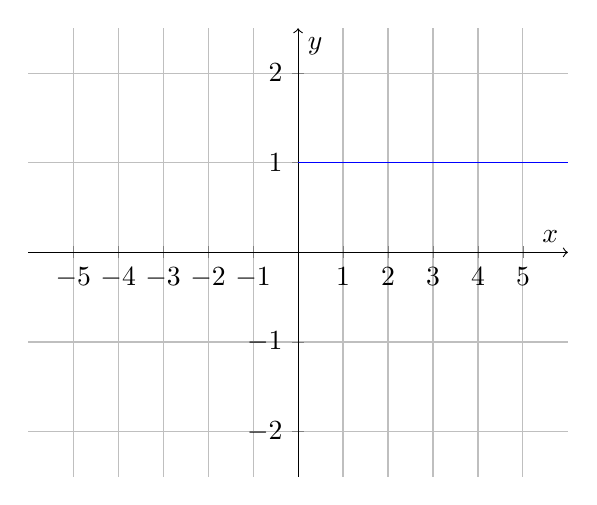
\begin{tikzpicture}
    \begin{axis}[
        xlabel={$x$},
        ylabel={$y$},
        axis lines=middle,
        axis line style={->},
        xmin=-6,
        ymin=-2.5,
        xmax=6,
        ymax=2.5,
        xtick={-5,-4,-3,-2,-1,0,1,2,3,4,5},
        ytick={-2,-1,0,1,2},
        legend style={at={(0.95,0.95)},anchor=north east},
        grid=both
      ]
        \addplot[domain=0:10, samples=100, color=blue]{1};
    \end{axis}
\end{tikzpicture} \\

\begin{equation*}
    |y| = \begin{cases}
        \;1  & x>0 \\
        \;0 & x \leq 0
    \end{cases}
\end{equation*}


discussing the concept of a "step function" in the context of neural networks and how it's used to model the behavior of neurons. Let me break it down for you:

\begin{itemize}
    \item In the brain, neurons are the basic functional units. They receive input signals from other neurons and, if the sum of those inputs reaches a certain threshold, the neuron "fires" or activates, transmitting a signal to other neurons. This activation is like turning on a switch, and it's a fundamental concept in neural activity.
    \item Step  When designing artificial neural networks (like those used in machine learning and deep learning), we often want to model the behavior of biological neurons. In this context, the "step function" is a simple mathematical function used to mimic the behavior of neurons.
    \item Think of the step function as an "on-off switch." If the input to the step function exceeds a certain threshold, the function's output is "on" (1), and if the input is below the threshold, the output is "off" (0). This behavior closely resembles the way biological neurons work, as they either fire or do not fire.
    \item The term "step" in the step function comes from the shape of its graph. When you plot this function on a graph, it looks like a step, where the output suddenly changes from 0 to 1 (or vice versa) at a specific threshold value.
\end{itemize}

In the previous function, x represents the input to the neuron, and \textbf{threshold}(whether the input is smaller or bigger than 0) is the value at which the neuron "fires." If x is less than the threshold, the output is 0 (off), and if x is greater than or equal to the threshold, the output is 1 (on).
In other words
For a step function, if the neuron’s output value, which is calculated by $sum(inputs\cdot weights)$
$+ bias$, is greater than 0, the neuron fires (so it would output a 1). Otherwise, it does not fire
and would pass along a 0. The formula for a single neuron might look something like:

